\documentclass[aspectratio=169]{beamer}
\usepackage{adjustbox}
\usepackage[utf8]{inputenc}
\usepackage{tikz}
\usepackage{hyperref}
\usepackage{multimedia}
\usepackage{ulem}
\usepackage{wasysym}
\usetikzlibrary{mindmap,trees}
\usepackage{siunitx}

\usepackage{pbox}
\usepackage{colortbl}

\usepackage[absolute,overlay]{textpos}

% \usetikzlibrary{mindmap,trees}

\usepackage{smartdiagram}
\usetikzlibrary{shapes.geometric,calc}
\usetikzlibrary{shapes.symbols}
\usetikzlibrary{shapes.symbols,positioning}
\usepackage{metalogo}

\usetikzlibrary{backgrounds, calc, shadows, shadows.blur}

\newcommand\addcurlyshadow[2][]{
    % #1: Optional aditional tikz options
    % #2: Name of the node to "decorate"
    \begin{pgfonlayer}{background}
        \path[blur shadow={shadow xshift=0pt, shadow yshift=0pt, shadow blur steps=6}, #1]
        ($(#2.north west)+(.3ex,-.5ex)$)
        -- ($(#2.south west)+(.5ex,-.7ex)$)
        .. controls ($(#2.south)!.3!(#2.south west)$) .. (#2.south)
        .. controls ($(#2.south)!.3!(#2.south east)$) .. ($(#2.south east)+(-.5ex,-.7ex)$)
        -- ($(#2.north east)+(-.3ex, -.5ex)$)
        -- cycle;
   \end{pgfonlayer}
}


%%%%%%%%%%%%%%%%%%%%%%%%%%%%%%%%%%%%%%%%%%%%%%%%%%%%%%%%%%%%%%%%%%%
% Style modifications
%%%%%%%%%%%%%%%%%%%%%%%%%%%%%%%%%%%%%%%%%%%%%%%%%%%%%%%%%%%%%%%%%%%

\usetheme{Berlin}

%%% Fonts %%%

% Change font. Fontspec requires xelatex instead of pdflatex!
% Font catalog: https://www.tug.dk/FontCatalogue/
% \usepackage{fontspec}

%\setsansfont{Comfortaa}
%\setsansfont{DejaVu Sans}
%\setsansfont{Fira Sans}

% Use "Fira Sans Light" as the normal font and the "Fira Sans" for
% bold fonts

%\setsansfont[
  %% ItalicFont={Fira Sans Light Italic},
  %% BoldFont={Fira Sans},
  %% BoldItalicFont={Fira Sans Italic}]{Fira Sans Light}

\setbeamerfont{title}{size=\Large, series=\bfseries}
\setbeamerfont{frametitle}{size=\large, series=\bfseries}


\usepackage{helvet}

%%% Slide template %%%

\setbeamertemplate{frames}[default]

% Empty headline / footline
\setbeamertemplate{headline}{}
\setbeamertemplate{footline}{}

% Remove navigation icons
\setbeamertemplate{navigation symbols}{}

%%% Colors %%%

\usecolortheme{crane}

\usecolortheme{crane}

\definecolor{lightgray}{RGB}{220,220,220}
\definecolor{darkgray}{RGB}{45,45,45}
%\definecolor{darkblue}{RGB}{0,86,137}
%\definecolor{darkblue}{RGB}{22,90,151}
\definecolor{lightblue}{RGB}{229, 245, 255}

%\definecolor{darkblue}{RGB}{1,1,100}


% Use the slide background in block environments                                                                                                      
\setbeamercolor{title}{fg=white,bg=darkgray}
\setbeamertemplate{blocks}[default]
\setbeamercolor{block title}{bg=}
\setbeamercolor{block body}{bg=lightgray}
\setbeamercolor{frametitle}{fg=white,bg=darkgray}
\setbeamerfont{block body}{size=\large}
\setbeamercolor{itemize item}{fg=black}
\setbeamertemplate{itemize items}[circle]
\setbeamercolor{section number projected}{bg=darkgray,fg=white}
\setbeamercolor{section in toc}{fg=black}
\setbeamercolor{subsection in toc}{fg=darkgray}

\addtobeamertemplate{block begin}{\pgfsetfillopacity{0.8}}{\pgfsetfillopacity{1}}
\addtobeamertemplate{frametitle}{\pgfsetfillopacity{1.0}}{\pgfsetfillopacity{1}}
\addtobeamertemplate{title page}{\pgfsetfillopacity{1.0}}{\pgfsetfillopacity{1}}

% Command to place the test (e.g. citation) in the center of the footer
\newcommand{\setfootercentertext}[1]{
  \setbeamertemplate{footline}{
    \hspace*{\fill}
    \raisebox{3mm}[0mm][0mm]{
      \tiny{#1}}\hspace*{\fill}}
}

%%%%%%%%%%%%%%%%%%%%%%%%%%%%%%%%%%%%%%%%%%%%%%%%%%%%%%%%%%%%%%%%%%%
% Content
%%%%%%%%%%%%%%%%%%%%%%%%%%%%%%%%%%%%%%%%%%%%%%%%%%%%%%%%%%%%%%%%%%%

%------------------------------------------------------------------------------
\title{Supervised Machine Learning Methods}
%------------------------------------------------------------------------------

\author{\small Konrad U. Förstner}

\institute{ZB MED -- Information Centre for Life Science \& TH Köln}

\date{\scriptsize 
  Workshop \textit{Systems Biology: From large datasets to biological insight}\\ \ \\
  2021-05-21\\\ \\
  \href{https://creativecommons.org/licenses/by/4.0/}{\includegraphics[width=0.88cm]{images/creative_commons_attribute.png}}
}

\logo{
  \includegraphics[height=1.0cm]{images/ZBMED_2017_EN.pdf}
  \includegraphics[height=0.8cm]{images/logo_TH-Koeln_CMYK_22pt.eps}
}

\begin{document}

%\setbeamertemplate{background}{
  % \includegraphics[height=\paperheight]{images/flickr_normanbleventhalmapcenter_2710796662_mod.jpg}
%}

\begin{frame}{}
  \titlepage
\end{frame}
\logo{}

\setcounter{tocdepth}{1}
\begin{frame}{}
   \tableofcontents
\end{frame}

%%%%%%%%%%%%%%%%%%%%%%
\section{Introduction}
%%%%%%%%%%%%%%%%%%%%%%

\begin{frame}{}
   \tableofcontents[currentsection]
\end{frame}

\begin{frame}
  % \frametitle{Basic concept of supervised machine learning}
  \begin{block}{}
    \vspace{0.5cm}
    \ \ \ \
    \begin{minipage}{0.10\textwidth}
      \begin{center}
        
\includegraphics[width=1.6cm]{images/publicdomainvectors_target-plain.pdf}
      \end{center}        
    \end{minipage}
    \hfill
    \begin{minipage}{0.80\textwidth}
      After the lecture you should have a basic understanding of
      supervised machine learning approaches and potential
      applications in research.\\

      After the practical part you should be able to implement them
      with Python and the package scikit-learn.\\

      We will not cover the mathematical background. This is not
      needed at this level but recommended later.
    \end{minipage}
    \vspace{0.3cm}
  \end{block}
\end{frame}

\setbeamertemplate{background}{
  \includegraphics[width=\paperwidth]{images/pexels-thisisengineering-3861969.jpg}}
\setfootercentertext{
  \href{https://www.pexels.com/photo/photo-of-code-projected-over-woman-3861969/}{https://www.pexels.com/photo/photo-of-code-projected-over-woman-3861969/} -- CC0}
\begin{frame}
  \frametitle{}
\end{frame}
\setbeamertemplate{background}{}
\setfootercentertext{}


\setbeamertemplate{background}{
  \includegraphics[width=\paperwidth]{images/Tools_by_Todd_Quackenbush.jpg}}
\setfootercentertext{
      \href{https://commons.wikimedia.org/wiki/File:Toolkit_and\_tools\_(Unsplash).jpg}{
        https://commons.wikimedia.org/wiki/File:Toolkit\_and\_tools\_(Unsplash).jpg} -- CC0}
\begin{frame}
\end{frame}
\setbeamertemplate{background}{}
\setfootercentertext{}


\begin{frame}
  \begin{center}
    \includegraphics[width=4.8cm]{images/xkcd_ai_methodology_2x.png}\\ \ \\
    {\tiny
      \href{https://xkcd.com/2451/}{https://xkcd.com/2451/} CC-BY-NC by Randall Munroe
      }
  \end{center}
\end{frame}

\begin{frame}
  \begin{center}  
    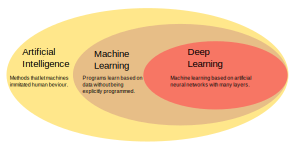
\includegraphics[width=13cm]{images/AI_ML_Deep_Learning.pdf}
  \end{center}    
\end{frame}


\begin{frame}
  \begin{center}
    \begin{adjustbox}{max totalsize={.9\textwidth}{.7\textheight},center}
    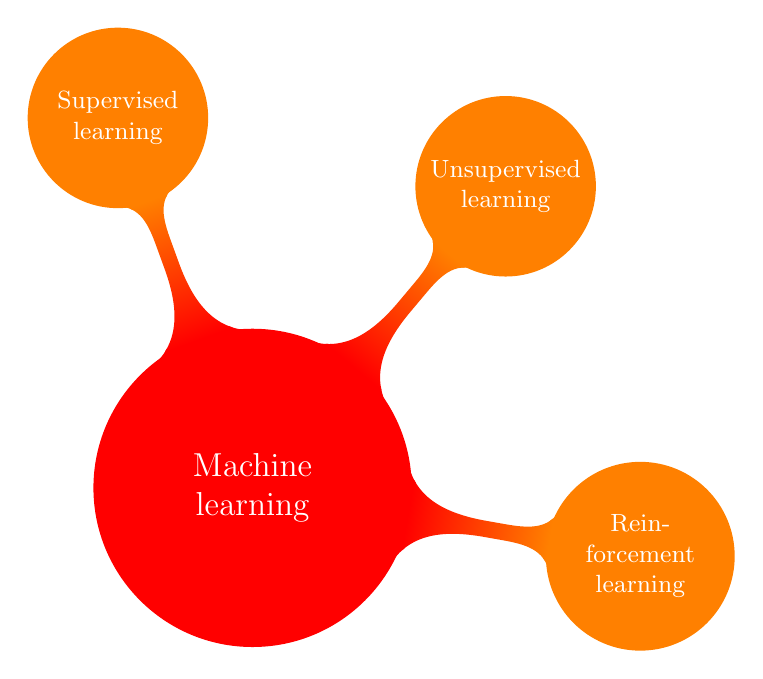
\begin{tikzpicture}
      \path[mindmap,concept color=red,text=white]
      node[concept] {Machine\\learning}
      [clockwise from=110]
      
      child[concept color=orange] { node[concept] {Supervised learning}}
      child[concept color=orange] { node[concept] {Unsuper\-vised learning}}
      child[concept color=orange] { node[concept] {Rein\-forcement learning}}

      ;
    \end{tikzpicture}  
    \end{adjustbox}
  \end{center}
\end{frame}

\begin{frame}
  \frametitle{Two types of tasks that can be solved with supervised learning}
  \begin{center}
    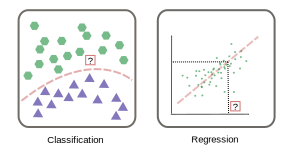
\includegraphics[width=13cm]{images/classification_and_regression.pdf}
  \end{center}
\end{frame}

\begin{frame}
  \frametitle{Classification types}
  \begin{center}
    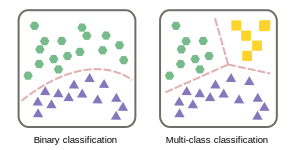
\includegraphics[width=13cm]{images/binary_vs_multi-class_classification.pdf}
  \end{center}  
\end{frame}


\begin{frame}
  % \frametitle{Basic concept of supervised machine learning}
  \begin{block}{}
    \vspace{0.5cm}
    \ \ \ \
    \begin{minipage}{0.10\textwidth}
      \begin{center}
        \includegraphics[width=1.6cm]{images/publicdomainvectors_Random-Alphabet-Brain.pdf}
      \end{center}        
    \end{minipage}
    \hfill
    \begin{minipage}{0.80\textwidth}
      Supervised learning means to generate models \\
      that generalize from given examples.
    \end{minipage}
    \vspace{0.3cm}
  \end{block}
\end{frame}


\begin{frame}
  \frametitle{Basic concept of supervised machine learning}

  \begin{block}{}
      \begin{center}
        \vspace{0.5cm}
      The model / function maps from a given two-dimensional matrix \textit{X}\\
      to an output vector \textit{y} with labels (classification)\\ or numerical values (regression).\\
      \ \\
      
      $X_{1} \rightarrow y_{1}$\\
      $X_{2} \rightarrow y_{2}$\\
      $X_{3} \rightarrow y_{3}$\\

      \end{center}
    \end{block}
\end{frame}


\begin{frame}
  % \frametitle{Basic concept of supervised machine learning}
  \begin{block}{}
    \vspace{0.5cm}
    \ \ \ \
    \begin{minipage}{0.10\textwidth}
      \begin{center}
        \includegraphics[width=1.6cm]{images/publicdomainvectors_Random-Alphabet-Brain.pdf}
      \end{center}        
    \end{minipage}
    \hfill
    \begin{minipage}{0.80\textwidth}
     In the actual training / learning process the parameters of the
     model / function are estimated. The model is then able to project
     the input variable $X$ to the output variable $y$.\\
     \begin{center}
       $y = f(X)$       
     \end{center}

    \end{minipage}
    \vspace{0.3cm}
  \end{block}
\end{frame}



\begin{frame}
  \frametitle{Example of classification}
  \begin{block}{}
    \vspace{0.5cm}
    \ \ \ \
    \begin{minipage}{0.10\textwidth}
      \begin{center}
        \includegraphics[width=1.6cm]{images/publicdomainvectors_Random-Alphabet-Brain.pdf}
      \end{center}        
    \end{minipage}
    \hfill
    \begin{minipage}{0.80\textwidth}

     \begin{center}
       Cancer classification based on single-cell\\
       gene expression data.
     \end{center}

    \end{minipage}
    \vspace{0.3cm}
  \end{block}
\end{frame}


\begin{frame}
  \frametitle{Example of regression}
  \begin{block}{}
    \vspace{0.5cm}
    \ \ \ \
    \begin{minipage}{0.10\textwidth}
      \begin{center}
        \includegraphics[width=1.6cm]{images/publicdomainvectors_Random-Alphabet-Brain.pdf}
      \end{center}        
    \end{minipage}
    \hfill
    \begin{minipage}{0.80\textwidth}

     \begin{center}
       Predicting the gene expression level of a gene based on the
       gene expression levels of several regulators.
     \end{center}

    \end{minipage}
    \vspace{0.3cm}
  \end{block}
\end{frame}

%%%%%%%%%%%%%%%%%%%%%%
\section{Concepts and terminology}
%%%%%%%%%%%%%%%%%%%%%%

\begin{frame}{}
   \tableofcontents[currentsection]
\end{frame}

\begin{frame}
  \frametitle{Entities and their features}  
  \begin{block}{}
    \vspace{0.5cm}
    \ \ \ \
    \begin{minipage}{0.10\textwidth}
      \begin{center}
        
\includegraphics[width=1.6cm]{images/publicdomainvectors_ftdissociatecell.pdf}
      \end{center}        
    \end{minipage}
    \hfill
    \begin{minipage}{0.80\textwidth}

      \textbf{Entities} (aka. samples, data points) are described by \\
      \textbf{features} (aka.  covariates, attributes) that have
      \textbf{values}.\\

      E.g. for different cell lines (entities) the relative expression
      (values) of several genes (features).
      
    \end{minipage}
    \vspace{0.3cm}
  \end{block}
\end{frame}

\begin{frame}
  \frametitle{Entities and their features}    
  \begin{block}{}
    \vspace{0.5cm}
    \ \ \ \
    \begin{minipage}{0.10\textwidth}
      \begin{center}
        
\includegraphics[width=1.6cm]{images/publicdomainvectors_ftdissociatecell.pdf}
      \end{center}        
    \end{minipage}
    \hfill
    \begin{minipage}{0.80\textwidth}

      Features can be\\
      \begin{itemize}
        \item categorical
          \begin{itemize}
          \item Nominal (e.g. cell line, cancer type, eye color, gender)
          \item Ordinal (e.g. very bad, bad, good, very good)
          \end{itemize}
        \item numerical
          \begin{itemize}
          \item Discrete (e.g. gene length in nucleotides, number cells)
          \item Continuous (e.g. cell length, concentration, relative expression) 
          \end{itemize}
      \end{itemize}
      
    \end{minipage}
    \vspace{0.3cm}
  \end{block}
\end{frame}

\definecolor{LightGray}{gray}{0.95}

\begin{frame}
  \frametitle{Feature selection}
  \begin{block}{}
    \begin{center}
      Choosing features with high variance.\\ \ \\

      {\small
        \newcolumntype{g}{>{\columncolor{LightGray}}c}
        \begin{tabular}{|g|c|c|g|c|}
          \hline
          \textbf{Feature A} & \textbf{Feature B} & \textbf{Feature C} & \textbf{Feature D} & \textbf{...}\\
          \hline
          10.00 & 5.01 & 102.01 & 120 & ... \\
          20.91 & 5.01 & 102.00 & 200 & ... \\
          80.03 & 5.01 & 102.09 & 980 & ... \\
          90.19 & 5.00 & 103.00 & 700 & ... \\
          50.99 & 5.02 & 102.31 & 703 & ... \\
          80.63 & 5.01 & 102.30 & 443 & ... \\          
          \hline
        \end{tabular}
      }
      
    \end{center}  
  \end{block}  
\end{frame}


\begin{frame}
  \frametitle{Feature scaling}
  \begin{block}{}

    \begin{center}
      Normalizing the feature values to their ranges e.g. min/max
      normalization, mean normalisation, standard score / z-score
      normalization.
    \end{center}
    
    \vspace{0.5cm}
    \hspace{1cm}
    \begin{minipage}{0.33\textwidth}
      {\small
        \begin{tabular}{|c|c|}
          \hline
          \textbf{Feature A} & \textbf{Feature B}\\
          \hline
          4.3 & 537\\
          5.3 & 703\\
          2.2 & 510\\
          1.5 & 200\\
          5.2 & 760\\
          \hline          
        \end{tabular}
      }
    \end{minipage}
    \begin{minipage}{0.08\textwidth}
      $\Rightarrow$
    \end{minipage}        
    \begin{minipage}{0.40\textwidth}
      {\small
        \begin{tabular}{|c|c|}
          \hline
          \textbf{Scaled Feature A} & \textbf{Scaled Feature B}\\
          \hline
          0.736 & 0.601\\
          1.000 & 0.898\\
          0.184 & 0.554\\
          0.000 & 0.00\\
          0.974 & 1.00\\
          \hline          
        \end{tabular}
      }
    \end{minipage}
    \hspace{1cm}
    \vspace{0.5cm}
  \end{block}
\end{frame}

\begin{frame}
  \frametitle{Features encoding}
  \begin{block}{}
    \begin{center}
      Translating categorical values into numerical values\\
      (e.g. via one-hot encoding)\\ \ \\

      {\small
        \begin{tabular}{|c|c|c|c|c|}
          \hline
          \textbf{} & \textbf{A} & \textbf{C} & \textbf{G} & \textbf{T}\\
          \hline
          A & 1 & 0 & 0 & 0 \\
          C & 0 & 1 & 0 & 0 \\
          G & 0 & 0 & 1 & 0 \\
          T & 0 & 0 & 0 & 1 \\
          \hline
        \end{tabular}

        \ \\ \ \\
        e.g. AATTGC becomes:\\ 
        %1000 1000 0001 0001 0010 0100\\
        \colorbox{white}{1, 0, 0, 0,}
        \colorbox{white}{1, 0, 0, 0,}
        \colorbox{white}{0, 0, 0, 1,}
        \colorbox{white}{0, 0, 0, 1,}
        \colorbox{white}{0, 0, 1, 0,}
        \colorbox{white}{0, 1, 0, 0}\\
      }
    \end{center}  
  \end{block}  
\end{frame}

\begin{frame}
  \frametitle{How well does the model fit?}

  \begin{block}{}
    \begin{center}
      \textbf{Overfitting}: Good performance on the training data,\\ poor
      generalization to other data\\      
    \end{center}
  \end{block}
  \begin{block}{}
    \begin{center}
      \textbf{Underfitting}: Poor performance on the training data\\ and
      poor generalization to other data\\
    \end{center}
  \end{block}
  
  \begin{block}{}
    \begin{center}
      \textbf{Regularization}: Different methods to prevent overfitting\\
    \end{center}
  \end{block}
\end{frame}

\begin{frame}
  \begin{center}
    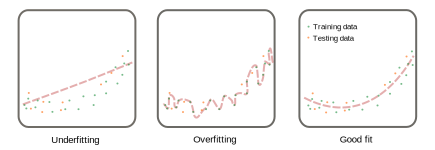
\includegraphics[width=14cm]{images/fitting_underfitting_overfitting.pdf}
  \end{center}    
\end{frame}
        
%% \begin{frame}
%%   \frametitle{Curse of dimensionality}
%%   \begin{block}{}
%%     \begin{center}
%%     \end{center}  
%%   \end{block}  
%% \end{frame}

%% \begin{frame}
%%   \frametitle{Evaluation of classificaions}
%%   Evaluation of binary classification - Confusion matrix for binary classification
%%   \begin{itemize}
%%   \item Positive (P): Observation is positive (for example: is an apple)
%%   \item Negative (N): Observation is not positive (for example: is not an apple).
%%   \item True Positive (TP): Observation is positive, and is predicted to be positive.
%%   \item False Negative (FN): Observation is positive, but is predicted negative.
%%   \item True Negative (TN): Observation is negative, and is predicted to be negative.
%%   \item False Positive (FP): Observation is negative, but is predicted positive.
%%   \item Accuracy
%%     ACC = (TP + TN) / (P + N)
%%   \item Recall sensitivity,  true positive rate
%%     TPR = TP / P
%%   \item Precision /  positive predictive value
%%     PPV = TP / (TP + FP)
%%   \item F1 (aka F-measure, F-score) - harmonic mean of precision and recall
%%     F1 = 2 * (1 / (1/recall) + (1/recall))
%%   \end{itemize}
%% \end{frame}

\begin{frame}
  \frametitle{Workflow for parameter fitting and evaluation}
  \begin{block}{}
    \begin{center}
      \begin{itemize}
      \item[1.)] Split into training and test/validation set (e.g. 75\%/25\%)
      \item[2.)] Train model by estimating the parameters with the training set
      \item[3.)] Evaluate the performance by using the test/validation
        set \\(e.g. scored as accuracy)
      \end{itemize}
    \end{center}    
  \end{block}
\end{frame}


\begin{frame}
  \frametitle{Workflow with cross-validation}
  \begin{center}
    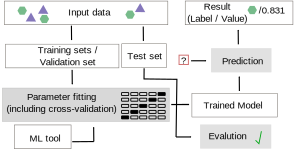
\includegraphics[width=14cm]{images/workflow_training_test_set.pdf}
  \end{center}    
\end{frame}


%%%%%%%%%%%%%%%%%%%%%%%%%%%%%%%%%%%%%%%%%%%%%%
\section{Selected supervised learning methods}
%%%%%%%%%%%%%%%%%%%%%%%%%%%%%%%%%%%%%%%%%%%%%%

\begin{frame}{}
   \tableofcontents[currentsection]
\end{frame}

\begin{frame}
  \frametitle{Overview of different methods}
  \begin{block}{}
    \begin{center}
      \begin{itemize}
      \item K-Nearest neighbor
      \item Naive Bayes
      \item Linear Regression
      \item Logistic Regression
      \item Decision trees
      \item Artificial Neural Network (multilayer perceptron)
      \item Genetic Programming
      \end{itemize}
    \end{center}    
  \end{block}
\end{frame}

%-------------------------------
\subsection{k-Nearest Neighbors}
%-------------------------------

\setcounter{tocdepth}{2}
\begin{frame}{}
   \tableofcontents[currentsubsection]
\end{frame}

\begin{frame}
  \frametitle{k-Nearest Neighbors}
  \begin{block}{}
    \begin{center}
      \begin{itemize}
      \item For classification and regression
      \item Simplest case of supervised machine learning
      \item Can be easily applied to multi-class classification
      \end{itemize}
    \end{center}
  \end{block}    
\end{frame}

\begin{frame}
  \frametitle{k-Nearest Neighbors}
  \begin{center}
    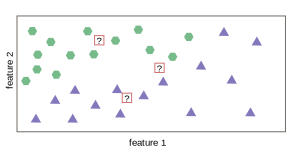
\includegraphics[width=13.0cm]{images/k_nearest_neighbour_classification_only_training_data.pdf}
  \end{center}
\end{frame}

\begin{frame}
  \frametitle{k-Nearest Neighbors}
  \begin{center}
    \includegraphics[width=13.0cm]{images/k_nearest_neighbour_classification_k_1.pdf}
  \end{center}
\end{frame}

\begin{frame}
  \frametitle{k-Nearest Neighbors}
  \begin{center}
    \includegraphics[width=13.0cm]{images/k_nearest_neighbour_classification_k_3.pdf}
  \end{center}
\end{frame}

\begin{frame}
  \frametitle{k-Nearest Neighbors}
  \begin{center}
    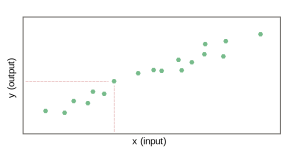
\includegraphics[width=13.0cm]{images/k_nearest_neighbour_regression_only_training_data.pdf}
  \end{center}
\end{frame}

\begin{frame}
  \frametitle{k-Nearest Neighbors}
  \begin{center}
    \includegraphics[width=13.0cm]{images/k_nearest_neighbour_regression_k_1.pdf}    
  \end{center}
\end{frame}

\begin{frame}
  \frametitle{k-Nearest Neighbors}
  \begin{center}
    \includegraphics[width=13.0cm]{images/k_nearest_neighbour_regression_k_3.pdf}
  \end{center}
\end{frame}


%-------------------------
\subsection{Linear models}
%-------------------------

\setcounter{tocdepth}{2}
\begin{frame}{}
   \tableofcontents[currentsubsection]
\end{frame}


\begin{frame}
  \frametitle{Linear models}
  \begin{block}{}
    \begin{center}
      $\hat{y} = w_{1}x_{1} + w_{2}x_{2} + w_{3}x_{3} + ... + w_{n}x_{n} + b$\\
      \ \\
      with $n$ as the  number of features\\
      $w$ are the different weights/coefficients\\
      $b$ the intercept\\
    \end{center}
  \end{block}  
\end{frame}

\begin{frame}
  \frametitle{Different ways to estimate the parameters}
  \begin{block}{}
    \begin{center}
      \begin{itemize}
      \item Ordinary Least Squares
        \begin{itemize}
        \item no parameters - easy to use but no possibility to adapt
        \end{itemize}
      \item Ridge
        \begin{itemize}
        \item coefficients should be close to zero
        \item more resistant against overfitting
        \end{itemize}    
      \item Least Absolute Shrinkage and Selection Operator (LASSO)
      \end{itemize}
    \end{center}
  \end{block}
\end{frame}

\begin{frame}
  \frametitle{Ordinary least squares (OLS)}
  \begin{center}
    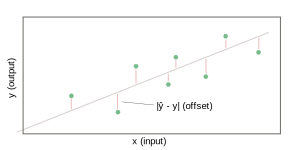
\includegraphics[width=13.0cm]{images/linear_model_ordinary_least_squares.pdf}
    Minimize the offset between $\hat{y}$ and $y$ the\\
    mean squared error (MSE) or sum of squared errors (SSE).
  \end{center}
\end{frame}


\begin{frame}
  \frametitle{}
  \begin{block}{}
    \begin{center}
      Once the parameters ($b$ and the weights $w$) of\\
      \ \\
      $\hat{y} = w_{1}x_{1} + w_{2}x_{2} + w_{3}x_{3} + ... + w_{n}x_{n} + b$\\
      \ \\
      are estimated the prediction can be performed\\
      by putting the x values of the data points into the\\
      equation to predict the y value.
    \end{center}
  \end{block}
\end{frame}

%-----------------------------------------
\subsection{Support Vector Machines (SVMs)}
%-----------------------------------------

\setcounter{tocdepth}{2}
\begin{frame}{}
   \tableofcontents[currentsubsection]
\end{frame}


\begin{frame}
  \frametitle{Support Vector Machines (SVMs) -- Separating hyperplane}
  \begin{center}
    \includegraphics[width=13.0cm]{images/svm_potential_separating_hyperplanes.pdf}
  \end{center}
\end{frame}

\begin{frame}
  \frametitle{Support Vector Machines (SVMs) -- Margin}
  \begin{center}
    \includegraphics[width=13.0cm]{images/svm_with_margin.pdf}
  \end{center}
\end{frame}

\begin{frame}
  \frametitle{Support Vector Machines (SVMs) -- Soft Margin}
  \begin{center}
    \includegraphics[width=13.0cm]{images/svm_with_soft_margin.pdf}
  \end{center}
\end{frame}

\begin{frame}
  \frametitle{Support Vector Machines (SVMs) -- Kernel trick}
  \begin{center}
    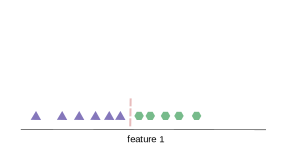
\includegraphics[width=13.0cm]{images/svm_kernel_trick_1.pdf}
  \end{center}
\end{frame}

\begin{frame}
  \frametitle{SVM -- Kernel trick}
  \begin{center}
    \includegraphics[width=13.0cm]{images/svm_kernel_trick_2.pdf}
  \end{center}
\end{frame}

\begin{frame}
  \frametitle{Support Vector Machines (SVMs) -- Kernel trick}
  \begin{center}
    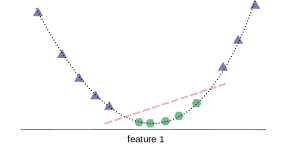
\includegraphics[width=13.0cm]{images/svm_kernel_trick_3.pdf}
  \end{center}
\end{frame}

%-------------------------
\subsection{Decision Trees and Random Forest}
%-------------------------

\setcounter{tocdepth}{2}
\begin{frame}{}
   \tableofcontents[currentsubsection]
\end{frame}


\begin{frame}
  \frametitle{Decision Trees}
  \begin{center}
    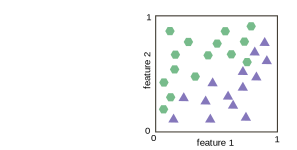
\includegraphics[width=13.0cm]{images/decision_tree_0.pdf}
  \end{center}  
\end{frame}

\begin{frame}
  \frametitle{Decision Trees}
  \begin{center}
    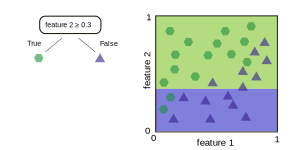
\includegraphics[width=13.0cm]{images/decision_tree_1.pdf}
  \end{center}  
\end{frame}

\begin{frame}
  \frametitle{Decision Trees}
  \begin{center}
    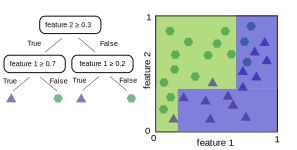
\includegraphics[width=13.0cm]{images/decision_tree_2.pdf}
  \end{center}  
\end{frame}

%% \begin{frame}
%%   Decision trees
%%   \begin{itemize}
%%   \item Concepts:
%%   \item node
%%   \item edge
%%   \item root
%%   \item leaf
%%   \item child
%%   \item parent
%%   \item A forest is a set of n ≥ 0 disjoint trees
%%   \item features: real-valued or categorial and also missing values
%%   \end{itemize}
%% \end{frame}

\begin{frame}
  \frametitle{Random forest}
  \begin{block}{}
    \begin{center}
      \begin{itemize}
      \item In the random forests approach many different decision
        trees are generated by a randomized tree-building algorithm.
      \item The training set is sampled with replacement to produce a
        modified training set of equal size to the original but with some
        training items included more than once.
      \item In addition, when choosing the question at each node, only a
        small, random subset of the features is considered.
      \item Decision is happening by presenting the data to all tree
        and then do a voting.
      \end{itemize}
    \end{center}
  \end{block}
\end{frame}

%--------------------------------------
\subsection{Artificial Neural Networks}
%--------------------------------------

\setcounter{tocdepth}{2}
\begin{frame}{}
   \tableofcontents[currentsubsection]
\end{frame}


\begin{frame}
  \begin{block}{}
    \begin{center}
      \frametitle{Artificial Neural Networks}
      \begin{itemize}
      \item Aka. Multilayer perceptrons or Feed-forward neural networks
      \item Inspired by natural neural networks
      \item For classification or regression
      \end{itemize}
    \end{center}  
  \end{block}  
\end{frame}


\begin{frame}
  \frametitle{Artificial Neural Networks}
  \begin{center}    
    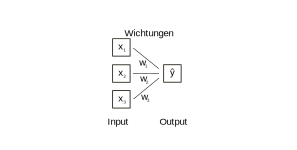
\includegraphics[width=13.0cm]{images/ANN_without_hidden_layer.pdf}
  \end{center}  
\end{frame}

\begin{frame}
  \frametitle{Artificial Neural Networks}
  \begin{center}
    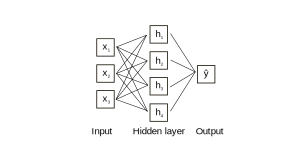
\includegraphics[width=13.0cm]{images/ANN_with_hidden_layer.pdf}
  \end{center}  
\end{frame}

\begin{frame}
  \frametitle{Artificial Neural Networks}
  \begin{center}
    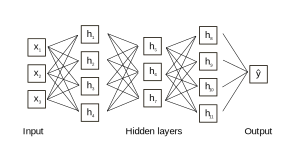
\includegraphics[width=13.0cm]{images/ANN_with_serveral_hidden_layers.pdf}
  \end{center}  
\end{frame}

\section{Summary}

\setcounter{tocdepth}{1}
\begin{frame}{}
   \tableofcontents[currentsubsection]
\end{frame}

\begin{frame}
  \frametitle{Summary}
  \begin{block}{}
    \begin{itemize}
    \item Supervised machine learning can be used for classification and
      regression.
    \item The parameters of models are estimated based on training data.
    \item Features have to be selected and potentially
      encoded or scaled.
    \item There are numerous machine learning approaches with different
      strength and weaknesses available.
    \end{itemize}
  \end{block}    
\end{frame}  

\setbeamercolor{block body}{bg=lightgray}
\setbeamertemplate{background}{
  \includegraphics[width=\paperwidth]{images/flickr_nateone_3768979925.jpg}}
\setfootercentertext{
  \href{https://www.flickr.com/photos/nateone/3768979925/}{https://www.flickr.com/photos/nateone/3768979925/}
  -- CC-BY by flick user
  \href{https://www.flickr.com/photos/nateone/}{nateone}}
\begin{frame}
  % \frametitle{Acknowledgements}
  \begin{block}{}
    \begin{center}
      \textbf{Thank you for your attention}\\
      \ \\
      \href{konrad.foerstner.org}{konrad.foerstner.org} / \href{https://twitter.com/konradfoerstner}{@konradfoerstner}\\
      \ \\
      \href{https://zbmed.de}{zbmed.de} / \href{https://twitter.com/ZB_MED}{@ZB\_MED} \\
      \ \\
      \href{https://th-koeln.de}{th-koeln.de} / \href{https://twitter.com/th\_koeln}{@th\_koeln}
      \ \\
      \ \\
      \includegraphics[height=1.8cm]{images/ZBMED_2017_EN.pdf} \ \ \ 
      \includegraphics[height=1.6cm]{images/logo_TH-Koeln_CMYK_22pt.eps}
      \\
    \end{center}
  \end{block}
\end{frame}


\end{document}
